\documentclass{article}
\usepackage{graphicx} % Required for inserting images
\usepackage[utf8]{inputenc}

\title{Dissertation}
\author{Jamie Day}
\date{October 2024}

\begin{document}

\maketitle
\section{Introduction}
\section{Background}

Effect handlers and the associated effects are a type of control flow pattern that have many applications, including for backtracking, cooperative multi-threading and more.\cite{effect_handlers_tutorial} A programmer will define specific \textit{effects}, and instantiate specific \textit{effect handlers} that will handle all effects of a predetermined type that are called within its scope. For example: 

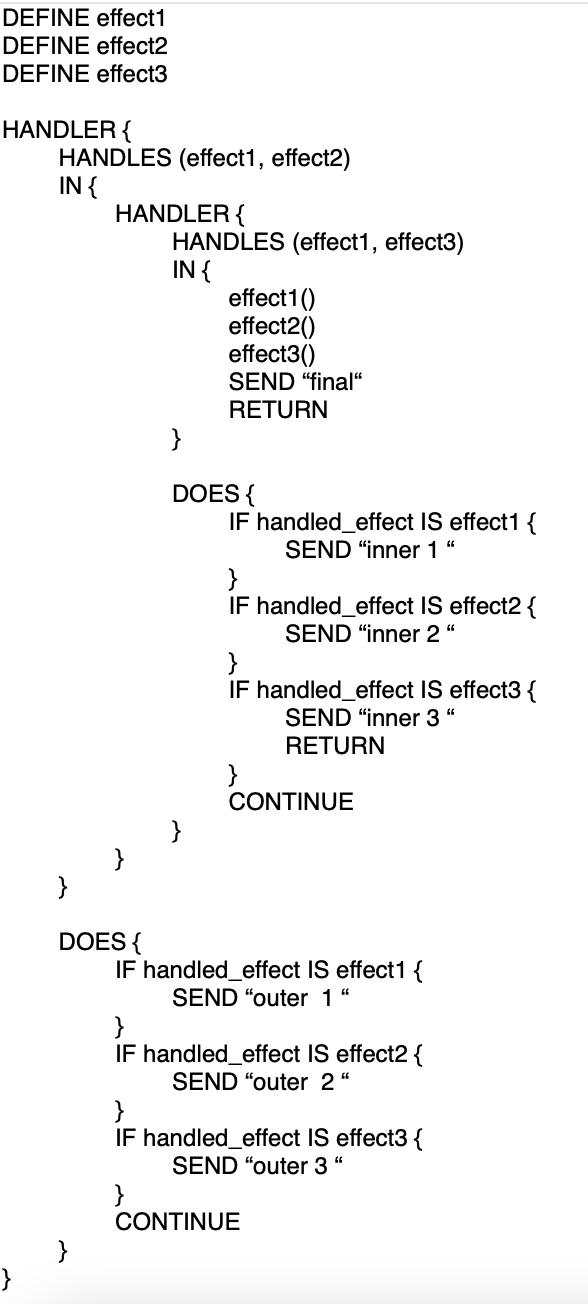
\includegraphics[scale=0.4]{pseudocode handler.png}

Here the output would be "inner 1 outer 2 inner 3 ". Note that this does not include the output "final" - the continuation does not have to be resumed after the error is handled. Note also that we can consider the second inner IF (that prints "inner 2 ") and the third outer IF to be dead code, since they don't handle this effect.

The key part to notice is what happens with effect 2 - the effect call "bubbles up" the stack of effect handlers until it finds a handler that can handle it. This is a key concept when it comes to effect handlers.

Note that since the inner handler does not handle the \textbf{[name]} effect, the effect call continues bubbling up the call stack until it finds the first handler that does handle it. This compositionality is essential to effect handlers usefulness %[rewrite this sentence].









Although much of the current usage of effect handlers is found in functional languages, there exist libraries that implement effect handling in almost every major language in which it is possible, including C. However, these libraries, such as \textbf{libmpeff}, are mostly designed specifically for compiler implementation, and as such offer features and make implementation decisions that do not necessarily make sense for the generic use case.\cite{libmprompt} \textbf{libseff}, on the other hand, is an implementation of effect handlers for C that is designed to be used by programmers directly.\cite{libseff_paper}

Currently defining an effect looks like this: %[image]

and calling it looks like this: %[image]

You may note that when defining the effect it is necessary to pass an integer id that defines the effect. This is a necessary detail of the current implementation of \textbf{libseff}: which effects a specific handler handles are stored as a single 64-bit integer, where each bit represents whether a handler represents that index of effect. This means that the number of IDs is limited to 64, meaning there can be at most 64 different  effects defined in a \textbf{libseff} program. This is the problem that this study will aim to solve.

This was implemented to increase speed at runtime, since this is a priority of the original \textbf{libseff} implementation. %[cite here]  

A further problem with this approach is that IDs must be independent even between libraries, which is unintuitive and generally makes including libraries that use libseff unnecessarily complicated, since it is necessary to ensure that the ids of effects do not collide, and the maximum limit of 64 effects may start to become relevant in this case.

This may cause unpredictable errors, since [cite 2.1 of the paper] errors are only caused when handlers with the same id are interlaced and then an effect is called that is meant to be handled by the handler higher in the heirarchy, but is handled by the lower one because the ids match. This doesn't cause an exception but fails silently and unpredictably which is a recipe for chaos. %[change this]

\bibliography{refs}
\bibliographystyle{plain}
\end{document}
